\documentclass[12pt]{article}
\textwidth 6.5in \textheight 9.0in \topmargin -.5in \oddsidemargin
0.0in \evensidemargin 0.0in

\usepackage{graphicx}
\usepackage[nogin]{Sweave}
\usepackage{tikz,pgflibraryshapes}
\usepackage{cite}
\usepackage{subfigure}
\usepackage[authoryear]{natbib}
\bibliographystyle{newapa}



\title{\textbf{Time-Inhomogeneous Multi-State Model for a Swine Flu Epidemic}}
\date{\today}

       \usepackage{amsmath,subfigure,alltt}
\setkeys{Gin}{width=0.5\columnwidth}


\newcommand{\comment}[1]{}

\comment{
}

\begin{document}

\maketitle


\section{Introduction}
\label{sec:introduction}

At the beginning of epidemics, such as H1N1 (``swine flu'') or severe acute respiratory syndrome (SARS), the major concern is the severity of the illness,
and the large number of individuals that have the potential to be hospitalized after being infected.  
Accordingly, during the early stages of an epidemic
we can assume that most cases are identified as ill individuals are encouraged to seek medical help and practitioners
to send samples to the labs for testing.  After the first few
weeks of an epidemic, testing of sick individuals is often discouraged to ease the burned on public health labs. 

In infectious disease modelling, we are often interested in estimating the case fatality ratio.  
That is, we are interesting in the proportion of cases
that eventually die from the disease.  However, crude rates calculated
throughout the epidemic often underestimate this quantity due to the large proportion of censoring present in the data.  The reason for this being that many 
individuals have yet to reach the terminal state of their illness, either recovery or death.
Additionally, these crude rates are often misleading due to shifts in case ascertainment which occur as the epidemic progresses because 
efforts from medical professionals become focussed on the more severe cases.  If these biases are not accounted for, they result in underestimation 
of the case fatality ratio (\cite{garske-bmj-2009}).  In fact, \cite{ghani-AmericanJournalEpi-2005}, even omit performing analyses during the first two months 
of the SARS epidemic due to a lack of data. 

We propose a Bayesian approach to this problem using time-inhomogeneous multi-state models.  This approach takes into account expert optinion which allows us to 
get reasonable estimates at the beginning an epidemic when the data are sparse.  The use of survival analysis is
a logical approach because this is the standard way of dealing with the large amounts of censoring present in the data.  We illustrate our approach through a simulation study
with the aim of appropriately estimating the fatality rate, predicting the hospital load and predicting the number of unobserved cases over the course
of the epidemic.  We are also interested in forecasting the number of
cases beyond the completion our simulated epidemic.  The strength of this method is appropriately estimating these quantities at the 
beginning of the epidemic while the data are sparse and censored, rather than at the completion.

We also compare our methods to similar analyses...


This remainder of this paper proceeds as follows.  Section \ref{sec:multiStateModel} goes into detail describing our multi-state model and Section \ref{sec:modelInference}
discusses model inference.  The results of our simulation study are shown in Section \ref{sec:simStudyResults}.  Finally, our conclusions
are given in Section \ref{sec:conclusions}.  


\section{Time-Inhomogeneous Multi-State Models}
\label{sec:multiStateModel}

\subsection{Infection Types}
\label{subsec:InfectionTypes}

We assumed that all individuals had one of three infection types:
mild, serious or deadly.  Individuals were classified as mild if
they recovered without needing to be hospitalized.  If an infection
was severe enough that hospitalization was required before recovery,
they were classified as having a serious infection type. Individuals
with a deadly infection, as the name suggests, were those that died
following hospitalization. For mild, serious and deadly cases,
respectively, we modelled the disease progression as follows:

\begin{equation}
\mbox{Infection} \stackrel{f_I(t)}{\Longrightarrow} \mbox{Onset} \stackrel{f_{OM}(t)}{\Longrightarrow} \mbox{Medical}  \stackrel{f_{MR}(t)}{\Longrightarrow} \mbox{Recovery} \label{eq:mildProgress}
\end{equation}

\begin{equation}
\mbox{Infection} \stackrel{f_I(t)}{\Longrightarrow} \mbox{Onset} \stackrel{f_{OS}(t)}{\Longrightarrow} \mbox{Medical} \stackrel{f_{SH}(t)}{\Longrightarrow} \mbox{Hospitalization} \stackrel{f_{SR}(t)}{\Longrightarrow} \mbox{Recovery} \label{eq:seriousProgress}
\end{equation}

\begin{equation}
\mbox{Infection} \stackrel{f_I(t)}{\Longrightarrow} \mbox{Onset} \stackrel{f_{OD}(t)}{\Longrightarrow} \mbox{Medical} \stackrel{f_{HD}(t)}{\Longrightarrow} \mbox{Hospitalization} \stackrel{f_{D}(t)}{\Longrightarrow} \mbox{Death}
\label{eq:deadlyProgress}
\end{equation}

Regardless of an individual's infection type, progression from one
stage to the next occurred according to a Weibull distribution with
parameters that corresponded to the respective transition and
infection type. Note that until an individual died or recovered
their infection type was unknown.  We also assumed that a small
proportion of mild cases were lost to follow up. That is, they
received medical consultation, and were assumed to recover since no
further information was available.

In this analysis, we assumed that the infection type probabilities varied with respect to age which we generated using log-linear cubic splines.  
This will be discussed further in Section \ref{subsec:infectionTypeProbs}.

\subsection{The Model}
\label{subsec:theModel}

We used a zero-inflated rounded Weibull for the time-to-event
distribution, denoted $f(t)$.  We used a rounded distribution
because the data only included the date the event took place. For
example, if there was an event recorded as being on the first day of
the epidemic, the event would actually have occurred at some point
between day 0.5 and day 1.5. To account for the large number of
administrative zeros recorded in the data, we used a zero-inflated
distribution.  That is, we let $\delta$ be the probability of
transitioning immediately to the death stage for an administrative
reason, such as arriving dead at the hospital. Furthermore, if we
let $Z$ denote the random variable for administrative zeros, we can
assume $Z$ follows a Bernoulli distribution with probability
$\delta$ and hence,

\begin{align*}
\text{Pr}(T=t|Z=1) =&\text{ }0 \text{ with probability } 1
\end{align*}

\noindent For the case where the individual was not an
administrative zero

\begin{align*}
\text{Pr}(T=t|Z=0) =&  \text{Pr}[\max(t-0.5,0) < y < t+0.5]\\
y \sim & \text{Weibull}\left [\frac{\mu}{\Gamma(1 + 1/\nu)}, \nu
\right]
\end{align*}

\noindent where $\mu = \mbox{E}[T = t|Z = 0]$ is the average time to
an event and $\nu$ is the Weibull shape parameter. We used beta
priors for the zero-inflation parameters and gamma priors for the
Weibull mean and shape parameters.

\subsection{Infection Type Probabilties}
\label{subsec:infectionTypeProbs}

As mentioned above in Section \ref{subsec:InfectionTypes}, we assumed the infection type probabilities varied with respect to age 
and generated them using log-linear cubic splines.  For individual $i$ we let $W_i$ $\in$ \{$M$, $S$, $D$\}
denote the infection type, where $M$, $S$ and $D$ represent mild,
serious and deadly infections, respectively and $X_i$ represents the
individual's age. The fatality rate is the marginal probability
$\mbox{Pr}(W_i = D) = g_D(X_i)$ and the non-fatal hospitalization
rate is the conditional probability $\mbox{Pr}(W_i = S|W_i \neq D)=
g_S(X_i)$  where $g_D$ and $g_S$ are log-linear cubic splines with
fixed knots and random coefficients that vary smoothly with age.  Note that this was done using the R package, DPpackage.


 \begin{figure}[!h]
 \begin{center}
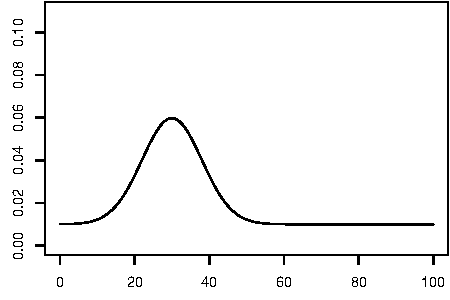
\includegraphics{Figures/G-ageVaryingDeadly}
 \end{center}
 \caption{Death probabilities.}
 \label{fig:ageVaryingDeadly}
 \end{figure}
   
\subsection{Discussion of Prior Distributions}         
        
\section{Model Inference}
\label{sec:modelInference}

Inference for this model was done through data augmentation and
random walk Metropolis simulations for calculating event time
parameters and predicting the number of unobserved cases.  We also forecasted the number of cases beyond the end of the simulated epidemic.


\subsection{Data Augmentation}
\label{subsec:dataAugmentation}

In order to deal with the censoring, we performed data augmentation
to impute the lifetimes as follows:

\begin{enumerate}

\item choose starting values for the probabilities

\item simulate $[W_i = D ] \sim \mbox{Bernoulli}(p_i)$, where $p_i = \mbox{Pr}(W_i = D | T_i > k_i; X_i)$,
 $k_i$ is the number of days previous that individual $i$ was hospitalized and $X_i$ is the age of individual $i$

\item simulate $[g_D|W_1, \ldots, W_n]$ to update
the parameters

\end{enumerate}

\subsection{Event Time Parameters}
\label{subsec:eventTimeParams}

After the data augmentation step, the likelihood was straightforward
to calculate since the observations were assumed to be independent.
Moreover, we could easily use random walk Metropolis to calculate
the event time parameters.
 If we denote $\theta$ as the current step and $\phi$ as
the proposed value, then $q(\theta, \phi)$ is the proposal
distribution for moving from the current position $\theta$ to the
proposed position $\phi$. For this simulation the proposal
distribution was absolute normal. The acceptance probability for the
random walk was:

\begin{eqnarray*}
\alpha(\theta, \phi) =  \mbox{min}\left\{1,
\frac{\pi(\phi)}{\pi(\theta)}\right\}
\end{eqnarray*}

\noindent where $\pi(^.) \propto \ell(^.) p(^.)$.  Using this
notation $p(^.)$ is the prior distribution, $\ell(^.)$ is the
likelihood and
 $\pi(^.)$ is the posterior distribution.  We accepted the move if $u \leq \alpha$ where $u \sim \mbox{Unif}(0, 1)$ and rejected otherwise.


\subsection{Number of Unobserved Cases}
\label{subsec:unobservedCases}

Again, we used random walk Metropolis to calculate the number of
unobserved infections.  We let $y_j$ denote the number of observed
cases on day $j$ of a $J$ day epidemic and we assumed that for each day of
the simulation:

\begin{eqnarray*}
y_j \sim \mbox{Binomial} (N_j, p_j), j = 1, \ldots, J
\end{eqnarray*}

\noindent where $N_j$ is the total number of cases (including both
observed and unobserved) on the $j^{th}$ day of the epidemic and
$p_j$ is the probability of observing a case on day $j$. A Poisson
prior with mean $\lambda_{j}$ is used for $N_j$, where
$\lambda_{j}$ is $[N_{j_{\mbox{inf}}} \theta + \omega]\gamma\mbox{ , }j = 1, \ldots, J$.  Using this notation, $N_{j_{\mbox{inf}}}$ is the number of infective individuals on the $j^{th}$ day of the epidemic,
$\theta$ is the rate parameter, $\omega$ is the immigration parameter and $\gamma$ is the probability of the case being mild, serious
or deadly.   

For this simulation, we accepted the proposed value with
probability:

\begin{eqnarray*}
\alpha(\theta, \phi) = \mbox{min} \left\{1, \frac{\pi(\phi)q(\phi,
\theta)}{\pi(\theta)q(\theta, \phi)} \right\}
\end{eqnarray*}

\noindent where $\pi(^.)$ is the posterior distribution and
$q(\theta, \phi)$ is the Poisson proposal distribution for day $j$ with mean $N_{j-1}$ + \pi_0$, where $\pi_0$ 
denotes the proposal offset or the mean increase in the number of new cases each day of the epidemic.  Note that for this simulation $q(\theta, \phi)$ is the 
conditional distribution, given $N_j$ is greater than $y_j - 0.5$.  Hence, in order for $q(\phi, \theta)$ to be a
valid probability density function we divided the conditional distribution by $P(Y_j > N_{j-1} + \pi_0)$,  where $Y_j$ are the 
individuals that have been infected, but have not had their medical consultation by day $j$. 
Similary, for $q(\theta, \phi)$, we divided by $P(Y_j > N_j + \pi_0)$.  
We accepted the proposed value if $u
\leq \alpha$ where $u \sim \mbox{Unif}(0,1)$.

Once this was complete, we performed data augmentation to estimate the progression of the cases from stage to stage by infection type as described in the 
multi-state models, \ref{eq:mildProgress} - \ref{eq:deadlyProgress} (Section \ref{subsec:InfectionTypes}).


\subsection{Forecasting the Number of Cases}
\label{subsec:forecasting}

The final goal of this paper was to predict the cases for a number of days beyond the completion of a simulated epidemic.  For a $J$ day
epidemic, if we denote $N_k$, $k$ = $J+1, \ldots, K$, as the number of cases on the $k^{th}$ day of the epidemic.  Then,

\begin{eqnarray*}
N_{k} \sim \mbox{Poisson}([N_{k_{\mbox{inf}}} \theta + \omega]\gamma), k = {J+1}, \ldots, K
\end{eqnarray*}

\noindent with $N_{k_{\mbox{inf}}}$, $\theta$, $\omega$ and $\gamma$ as defined in Section \ref{subsec:unobservedCases}.  Note that these forecasts were done separately
for each infection type.  Once this was complete, we performed data augmentation, as discussed in Section \ref{subsec:dataAugmentation}. 

                                                                                                                                              
\section{Results of the Swine Flu Simulation Study}
\label{sec:simStudyResults}

This section summarizes the results of a simulated 20 day epidemic and then forecasted the number of cases for the next 10 days beyond the end of the
epidemic. 


\subsection{Fatality Rate}
\label{subsec:fatalityRate}

\end{document}